\section{Methods}\label{sec:methods}

% =========================================================================
%

\subsection{Convolutional neural networks}

Fully-connected feed-forward neural networks (FCNN) can be used for a variety of tasks, including image recognition. However, these require flattening of the input data, which means that you may lose important characteristics when working with images, like the position of the pixel and the value of adjacent pixels. It is instead common to use convolutional neural networks (CNN), which keep these features, for image classification tasks. In a CNN, you create a feature map from your image where each element is just connected to a small group of pixels, in contrast to a FCNN where all nodes are connected \cite{raschka:2022:ml_pytorch_scikit}.

CNNs are based on the mathematical concept of convolution 

A CNN consists of several types of layers, most often a series of convolutional and pooling layers followed by one or more fully-connected layers. In a convolutional layer, a $n \times n$ filter with weights applies a convolution or cross-correlation operation to the input data, reducing the size of the original image. This process can be visualized as the filter "moving across" the image, calculating a weighed sum of a $n \times n$ subset of pixels, before moving to the next subset of pixels with step size (stride) $S$ (with or without overlap, depending on $n$ and $S$) \cite{dumoulin2016guide}. In this process, the center pixels are included in several of the summations, while the corners only get used once. To avoid over-emphasizing the center pixels compared to the edges, it is common to pad the input data with zeros at the ends, where the number of padding values are specified with the parameter $p$ \cite{raschka:2022:ml_pytorch_scikit}. The size of the filter $n$, stride $S$ and padding $p$ are all hyperparameters of the model that can be tuned.

After a convolution step, the output is transformed with an activation function, commonly the ReLU function
\begin{equation}
    f(x) = \max(0,x).
\end{equation}
The dimensionality of the output of the activation is then further reduced by pooling. The pooling takes subsets of the data (without overlap), and reduces it to a single value either by using the maximum value (max pooling) or mean (average pooling) of the subset. The ReLU and pooling functions have no trainable parameters.

It is common to apply several steps of convolution, ReLU and pooling. After this, the output is flattened to 1 dimension and used as input a FCNN. For classification, the output layer of the FCNN commonly uses softmax activation, and has the same size as the number of categories.

Training CNNs, and transfer learning

% EB writes here - this is method but parts of it can also be included in introduction.

\subsection{Vision Transformers} \label{ssec:vit}
\subsubsection{The origin of transformers}
In 2017, a novel architecture for deep learning was introduced with the infamous article 
"Attention is all you need" \cite{attention}. This architecture is today known as the 
transformer, and it formed the basis for the current AI wave which includes major 
names such as ChatGPT, Dal-E and AlphaFold 2.

The transformer architecture was originally thought to replace recurrent neural networks (RNN)
as the model of choice for translation of text. The model had several novel ways to train a network,
but the main focus was on the self-attention mechanism. 

\subsubsection{Self-attention mechanism}
For a transformer with text inputs, each word in the text are considered tokens. When fed into the model, each token produces it's own embedding vector in space, $\vec{E}_i$ for $i = {1, 2, ..., n}$. Then, key $\vec{K}_i$ and query $\vec{Q}_i$ vectors are found using weight parameters for each vector
\begin{equation}
    \begin{split}
    \vec{Q}_i = W_Q \vec{E}_i  \\
    \vec{K}_i = W_K \vec{E}_i . \\
    \end{split}
\end{equation}
Each of these vectors combined make out the key and query matrices $K$ and $Q$. If we find
\begin{equation}
    Attention\ map = QK^T,
\end{equation}
this attention map tells us which embeddings attend to each other - or said differently, which tokens that are likely to be in the same context. The attention map as it's shown here is simply an $n x n$ matrix that describe how tokens relate to each other by the size of the computed dot product between 
\begin{equation}
   A_{i, j} =  W_Q \vec{E}_i \ \cdot \ W_K \vec{E}_j, 
\end{equation}
where $A_{i, j}$ is an element in the attention map. 

The original authors refer to their attention mechanism as a "Scaled Dot-Product Attention", which they present mathematically as
\begin{equation}
    Attention(Q, K, V) = \frac{QK^T V}{\sqrt{d_K}}.
\end{equation}
The $d_K$ represents the dimension for matrix $K$ (which is equal to the dimension of $Q$), and the scalar $\frac{1}{\sqrt{d_K}}$ constitutes the "scaled" part of the "Scaled Dot-Product Attention", and authors state it was added for numerial stability. This new matrix $V$ is a concatenation of a set of value vectors $\vec{V}_i = W_V\vec{E}_i$. If we then find
\begin{equation}
    \Delta\vec{E}_i = \vec{V}_i A_j  
\end{equation}
for all combinations of $i$ and $j$ so that each value vector is multiplied with each column of the attention map, the resulting term $\Delta\vec{E}_i$ is what we use to update the embedding of the original token so that $\vec{E}_i  = \Delta\vec{E}_i + \vec{E}_i $. 

During training of a ViT, all the weight matrices $W_K, W_Q , W_V$ get continuously updated so that the embeddings are shaped into more contextualized tokens. Most attention heads then feed their updated embeddings into an MLP network for later classification or regression. 

This description of the transformer self-attention mechanism has skipped a few steps such as the masking of the attention map as well as the positional embedding process. We have tried to best explain the very distinct functionality for a single transformer attention head. It should be noted that most transformers have several attention heads performing this computation in parallel. 

\subsubsection{The origin and function of vision transformers}
Only three years after the first transformer architecture was introduced, the article 
"An Image is Worth 16x16 Words: Transformers for Image Recognition at Scale" \cite{first_vit}
introduced the first functional transformer trained on images, and it was baptized as a Vision
Transformer (or ViT for short). The authors demonstrate how a ViT outperforms classical 
deep learning methods such as convoultional neural networks (CNN). 

A ViT splits an image into even sized, non-overlapping patches, which are then linearly embedded
as token representations. These tokens are then fed into the regular transformer architecture. The previously mentioned attention mechanism is then used during training
so that the model considered spatial relationships within and between patches. 

The authors of this 
report will not pretend to understand the ViT completely, but we provide the reader with all sources
to fully comprehend this architecture, and present the original layout of a ViT in Figure \ref{fig:ViT}

\begin{figure}[H]
    \centering
    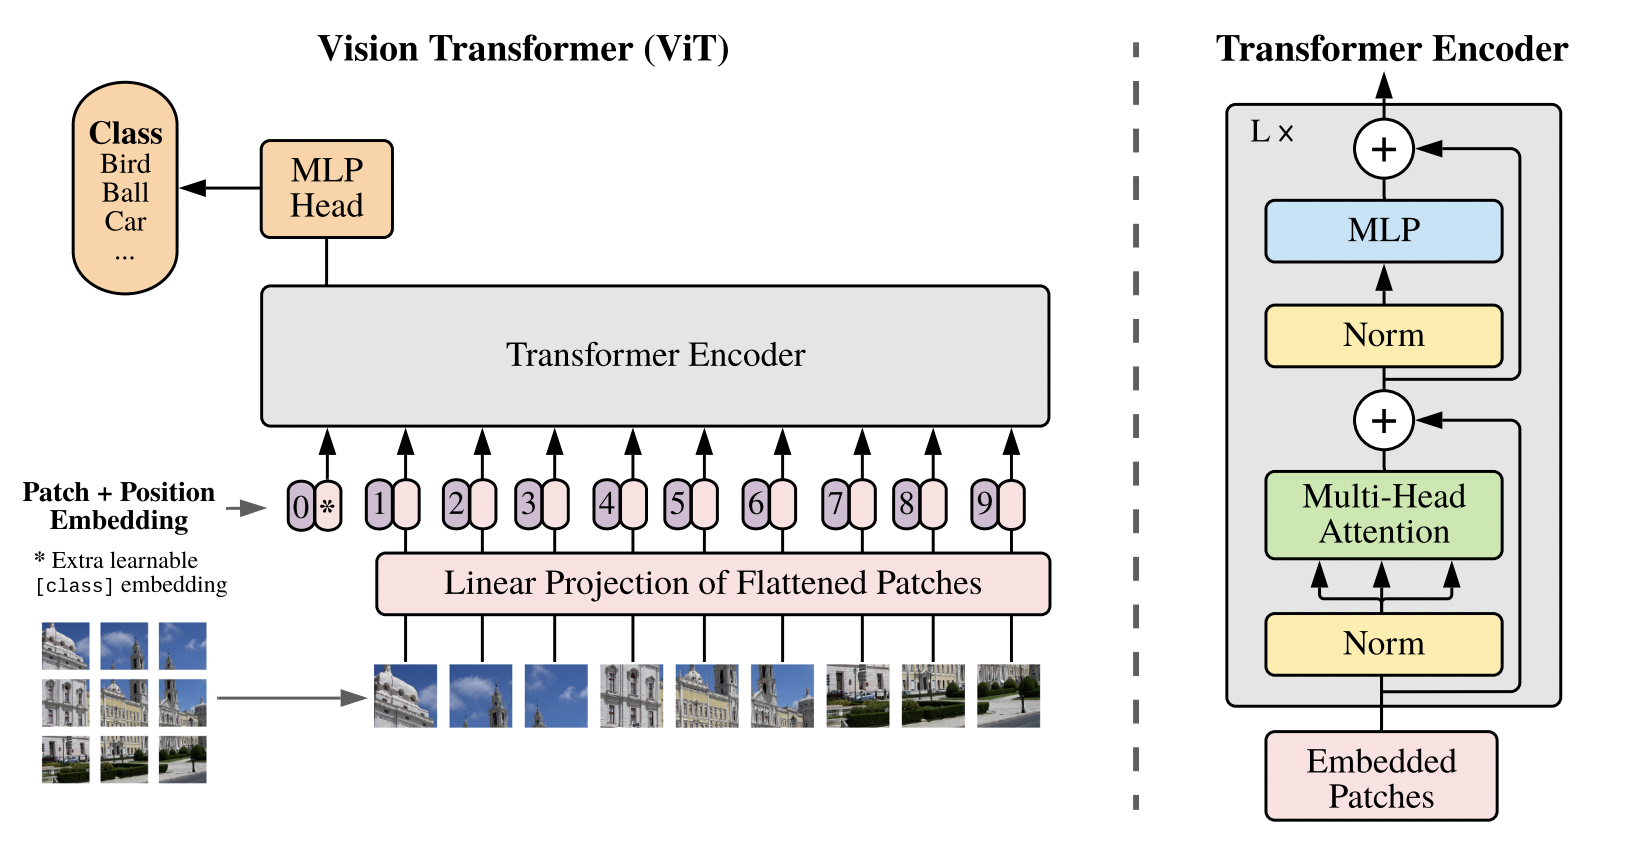
\includegraphics[width=1\linewidth]{examples/tests_eb/figs/vit.png}
    \caption{Vision Transformer layout as presented from it's original paper by Dosovitskiy et. al \cite{first_vit}. The Multi-Head attention layer is what we've previously described as a self-attention layer. The MLP layer stands for Multi Layer Perceptron, this is the same as FCNN.}
    \label{fig:ViT}
\end{figure}

\subsubsection{Self-\textbf{di}stillation with \textbf{no} labels (Meta's \textbf{DINO})} \label{sssec:dino}
The first DINO was introduced by Facebook (now Meta) shortly after the original ViT was proposed \cite{dino1}, as a self-supervised computer vision method inspired by the "Bootstrap your own latent"-method of self-supervision \cite{byol}. The authors found that DINO works exceptionally well with ViT architechtures, and their model achieved 80.1\% top-1 on ImageNet in linear evaluation.  

The self-\textbf{di}stillation aspect refers to a teacher-student interaction, where a teacher model looks into global augmented crops of an image and the student model looks into both smaller (local), augmented crops and global, augmented crops of the same image patch. The goal is that both the student and the teacher gives us the same feature representation of the different crops, essentially teaching the model that minor deviations in size and color should still fall into the same representation. 

%
The DINO loss function formalizes this teacher-student relationship mathematically. For both the teacher and student models, respective feature vectors derived from the same image patch, but with different augmentations $x_1 \text{ and } x_2$ are extracted from the token of a ViT. These vectors are passed through the MLP to produce prototype scores, which are then turned into probabilities using the softmax function
\begin{equation}
\text{Softmax}(\mathbf{x_i}) = \frac{e^{x_i}}{\sum_{j} e^{x_j}}.
\end{equation}
We call the student probabilities \( p_1 \) and the teacher probabilities \( p_2 \). The loss function is then defined as:
\[
\mathcal{L}_{\text{DINO}} = -\sum p_2 \log p_1.
\]
To compute these probabilities, the prototype scores for the student are obtained by processing the student’s embedding vectors through a set of learned weight matrices. Similarly, the teacher’s embedding vectors are processed to generate its prototype scores, which are centered using a moving average. 

During training, the weight matrices of the student model are updated to minimize the loss, while the teacher’s parameters are updated using an exponential moving average (EMA) of the student’s weights. A simple figure that aims to illustrate this is shown in Figure \ref{fig:dino}, and an even better gif illustrates this on DINO's \hyperlink{https://github.com/facebookresearch/dino}{Github}.
%
%
%
\begin{figure}[H]
    \centering
    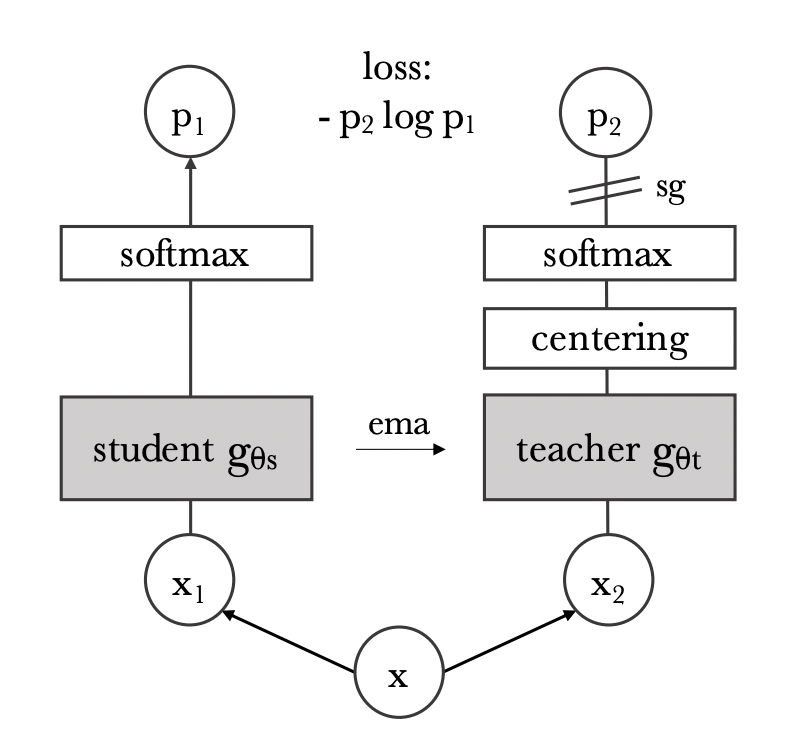
\includegraphics[width=0.7\linewidth]{examples/tests_eb/figs/dino.png}
    \caption{Student-Teacher interactions as presented in original DINO article \cite{dino1} for a single token. The gray boxes with $g\theta$ represent the shared architecture of the student and teacher, this can either be CNN or ViT. The ema function is an exponential moving average which is provided from the student to update the parameters in the teacher. The sg is a stop-gradient operator that ensures gradients are propagated only through the student.}
    \label{fig:dino}
\end{figure}
%
%


The original DINO's performance has improved with Meta's newest release of the updated \textbf{DINOv2} \cite{dino2} from january 2024. the model produces a set of 384 embeddings and has been trained on LVD-142M, meaning 142 million images. The authors themselves make the claim that the newest DINOv2 does not require any fine tuning, and we've therefore chosen to go for their reccomended approach. 

\begin{table}[H]
\centering
\caption{ViT architecture details for DINOv2 ViT-S}
\begin{tabular}{c|c}
\textbf{ViT Model} & DINOv2 ViT-S \\ \hline
Params & 21M params \\ 
Patch Size & 14 \\ 
Embedding Dimension & 384 \\
Attention heads & 6 \\ 
NN Architecture & MLP FFN \\
Training Data & LVD-142M \\ 
\end{tabular} \label{tab:vit-params}
\end{table}

We present the architecture of our chosen DINOv2 in Table \ref{tab:vit-params}. This is the same for student and teacher, but in the end it is the teacher parameters that we import to extract our feature embeddings. We went with one of their smaller models for this project, even though it has worse performance, in order to save some time when running the large data set. Their current best DINOv2 model is the ViT-g with 1.1B params, but this we save for later use.



\subsection{Dimensionality Reduction and Clustering}
We reduce the dimensionality of our ViT-derived feature and perform simple clustering methods on the reduced features. Our methods include Prinipal Component Analysis, Uniform Manifold Approximation and Projection for
Dimension Reduction and K-means clustering. 

\subsubsection{Principal Component Analysis (PCA)}
Consider a classic design matrix
$$
\boldsymbol{X}=\begin{bmatrix}
x_{0,0} & x_{0,1} & x_{0,2}& \dots & \dots x_{0,p-1}\\
x_{1,0} & x_{1,1} & x_{1,2}& \dots & \dots x_{1,p-1}\\
x_{2,0} & x_{2,1} & x_{2,2}& \dots & \dots x_{2,p-1}\\
\dots & \dots & \dots & \dots \dots & \dots \\
x_{n-2,0} & x_{n-2,1} & x_{n-2,2}& \dots & \dots x_{n-2,p-1}\\
x_{n-1,0} & x_{n-1,1} & x_{n-1,2}& \dots & \dots x_{n-1,p-1}\\
\end{bmatrix},
$$
where the rows $n$ represent our data points, or images, while the columns $p$ represent our features. This can be written as 
$$
\boldsymbol{X}=\begin{bmatrix} \boldsymbol{x}_0 & \boldsymbol{x}_1 & \boldsymbol{x}_2 & \dots & \dots & \boldsymbol{x}_{p-1}\end{bmatrix}.
$$
Here, each vector $\mathbf{x_i}$ for $i = [0, 1, \cdots, p-1]$ represents a feature, and all of the elements contained in the vector represent how a single data-point is described by that feature. If we then observe a mean centered covariance matrix written as 
$$
\boldsymbol{C}[\boldsymbol{x}] = \begin{bmatrix}
\mathrm{var}[\boldsymbol{x}_0] & \mathrm{cov}[\boldsymbol{x}_0,\boldsymbol{x}_1]  & \dots  & \mathrm{cov}[\boldsymbol{x}_0,\boldsymbol{x}_{p-1}]\\
\mathrm{cov}[\boldsymbol{x}_1,\boldsymbol{x}_0] & \mathrm{var}[\boldsymbol{x}_1]& \dots & \mathrm{cov}[\boldsymbol{x}_1,\boldsymbol{x}_{p-1}]\\
\mathrm{cov}[\boldsymbol{x}_2,\boldsymbol{x}_0]   & \mathrm{cov}[\boldsymbol{x}_2,\boldsymbol{x}_1] & \dots  & \mathrm{cov}[\boldsymbol{x}_2,\boldsymbol{x}_{p-1}]\\
\dots & \dots & \dots & \dots & \\
\mathrm{cov}[\boldsymbol{x}_{p-1},\boldsymbol{x}_0]   & \mathrm{cov}[\boldsymbol{x}_{p-1},\boldsymbol{x}_1]  & \dots  & \mathrm{var}[\boldsymbol{x}_{p-1}]\\
\end{bmatrix},
$$
we can re-write this as 
$$
\boldsymbol{C}[\boldsymbol{x}] = \frac{1}{n}\boldsymbol{X}^T\boldsymbol{X}= \mathbb{E}[\boldsymbol{X}^T\boldsymbol{X}]
$$
by the classic definition of the covariance matrix. We then move into the spectral theorem, where $\boldsymbol{A} = \boldsymbol{SDS^{-1} = SD S^T}$, and $\boldsymbol{S}$ is some orthogonal matrix. Then:
\begin{equation}
\begin{split}
    \boldsymbol{A^T} & = \boldsymbol{(S D S^T)^{T}} \\ 
    & = \boldsymbol{ (S^T)^T D^T S^T =  S D S^T = A}.
\end{split}
\end{equation}
Here, $\boldsymbol{A}$ is a symmetric matrix where there exists a basis for each finite dimensional vector space, and $\boldsymbol{D}$ is a diagonal matrix with the eigenvalues of $\boldsymbol{A}$ as it's signature. 
\\
\\
If we assume there exists a transformation $\boldsymbol{S}^T\boldsymbol{C}[\boldsymbol{x}]\boldsymbol{S}=\boldsymbol{C}[\boldsymbol{y}]$ so that the resulting matrix $\boldsymbol{C}[\boldsymbol{y}]$ is a diagonal matrix with the signature $\vec{\lambda}= [\lambda_0,\lambda_1,\lambda_2,\dots,\lambda_{p-1}]$, 
we can derive the following expression
\begin{equation}
\begin{split}
\boldsymbol{C}[\boldsymbol{y}] = \boldsymbol{S}^T\boldsymbol{C}[\boldsymbol{x}]\boldsymbol{S}. \\
\end{split}
\end{equation}
If we multiply the matrix $\boldsymbol{S}$ from the left on either side and consider that our matrix $\boldsymbol{C}[\boldsymbol{y}]$ is in fact a diagonal matrix written as $\boldsymbol{C}[\boldsymbol{y}], = \boldsymbol{I}\vec{\lambda} = \boldsymbol{\lambda }$, we're left with the expression
\begin{equation}
\begin{split}
\boldsymbol{S}\boldsymbol{C}[\boldsymbol{y}] & = \boldsymbol{C}[\boldsymbol{x}]\boldsymbol{S} \\
\boldsymbol{S} \boldsymbol{\lambda}\boldsymbol{S^T} & = \boldsymbol{C}[\boldsymbol{x}].
\end{split}
\end{equation}
% Consider putting all the math in appendix, tmi! 
\\
\\
When solving for a set of principal components, we wish to find the eigenvalues and eigenvectors of our covariance matrix $\boldsymbol{C[x]}$, where one principal component is an eigenvector $\vec{v_i}$ and the importance (or variance expained) by said vector is determined by the corresponding eigenvalue $\lambda_i$. This is then the same as solving the above equations for $\boldsymbol{\lambda}$ and $\boldsymbol{S}$, as the columns $\vec{s}_i$ in the latter are the corresponding eigenvectors to $\lambda_i$. Thus we're solving a set of equations

\begin{equation}
    \boldsymbol{C[x]} \vec{s}_i= \lambda_i\vec{s}_i.
\end{equation}
%
This is done through Single Value Decomposition (SVD) through existing libraries as we describle in our Tools section \ref{subsec:tools}. When discussing PCA, it is also important to introduce the term explained variance ratio, as we use this to illustrate the variance contribution from each eigenvector. The cumulative variance for a subset of eigenvalues $r+1$ from a total set of $n+1$ is written as
\begin{equation}
    cum\ variance(\lambda_0, \cdots, \lambda_r)  = \frac{\sum_{i = 0}^{i = r} \lambda_i}{\sum_{i = 0}^{i = n-1} \lambda_i}
\end{equation}



\subsubsection{Uniform Manifold Approximation and Projection for Dimension Reduction (UMAP)}
UMAP is a newer dimensionality reduction technique presented by Leland et. al 2020 \cite{umap}. The authors describe it as a cross-entropy minimization problem where a low-dimension topographical representation of the data $Y$ is altered to approximate a high-dimensional topographical dimension $X$.

In simple terms, the method first construct a set of fuzzy set approximations for both Y and X. A fuzzy set of $i$ enumerated elements from a carrier set $A$ has a map, or a membership function $u : A \rightarrow I$ where $u(x) \in [0, 1]$. This can also be interpreted as the degree of truth to the sentence "$x$ belongs to $A$". In cases where $u(x) \in \{0, 1\}$, we have a crisp set, while a fuzzy set can be written as $(A, u(x))$. 

UMAP is often presented as similar to t-SNE, as the dimensionality reduced embedding is optimized in a with respect to the fuzzy set cross entropy
\begin{equation}
\begin{split}
& \\
&C\left((A, \mu), (A, \nu)\right) \triangleq \\
&\sum_{a \in A} \left(\mu(a) \log \frac{\mu(a)}{\nu(a)} + (1 - \mu(a)) \log \frac{1 - \mu(a)}{1 - \nu(a)}\right).
\end{split}
\end{equation}
$(A, \mu)$ and $(A, \nu)$ are comparable fuzzy sets with different membership functions $\mu$ and $\nu$, taking in the enumerated elements $x$ from the original, shared carrier set $A$. The variable $a$ here is derived from the variable $x$, but we will not go into details on this. 

The fuzzy sets are then constructed as simpleces. A simplex is a way to build a $k$-dimensional object as illustrated in Figure \ref{fig:simpleces}. This combination results in what the authors refer to as "local fuzzy simplicial set representations". Finally, these representations are patched together to construct topographical representations of higher dimensional data. 

\begin{figure}[H]
    \centering
    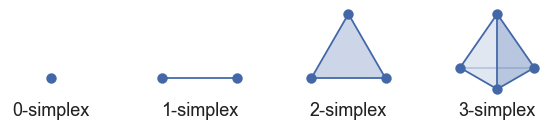
\includegraphics[width=1\linewidth]{examples/tests_eb/figs/Skjermbilde 2024-12-05 kl. 16.56.40.png}
    \caption{Simpeces illustrated here can be used to as combinatorial building blocks.}
    \label{fig:simpleces}
\end{figure}

One important thing to note about the UMAP is that it is optimized by stochastic gradient descent, and therefore clustering results are not reproducible. To work around this, we implemented the method with a set seed, even though the authors warn that might cause a slight reduction in performance. 

The full paper on UMAP is around 60 pages long, and we will not deny that the concepts of manifold approximations are a bit too advanced for us to do by hand. Luckily, UMAP is available as a package in Python and very user friendly. We expect the UMAP dimensionality reduction to capture a broader spectrum of variance and therefore include this as one of our unsupervised methods.

\subsection{Tools} \label{subsec:tools}
\subsection{Data} \label{subsec:data}

\subsubsection{Automated plankton imagers}

The models were applied to two sets of images from different imaging hardware (figure \ref{fig:plankton-img}). The first, PlanktoScope, is an automated quantitative plankton imaging system which can be built with a Raspberry Pi and standard parts \cite{pollina2022:planktoscope}. The imaging is based on a flow-through system, where the sample is pumped through a flat glass capillary and imaged, stopping the flow for every image to avoid distortion. The size range of the imaged objects is dependent on the camera quality and capillary width, and was in our setup constrained to objects between 40-200 µm. Although the imaging itself is automated, using the PlanktoScope is dependent on manually sampling for material, e.g., field sampling with a plankton net. The samples are backlit, resulting in images with a light background.

The other hardware is a Continuous Particle Imaging Classification System (CPICS), which is an in-situ plankton imaging system (\hyperlink{https://www.coastaloceanvision.com/cpics}{https://www.coastaloceanvision.com/cpics}). In contrast to the PlanktoScope, the CPICS is not dependent on manual sampling, but is deployed at the sampling site, imaging particles that flow past the camera. This allows for a higher throughput than the PlanktoScope, but constrains the data to a single location per deployment. The CPICS has a larger size range than the PlanktoScope (approx. 50 µm to several cm), but provides lower picture quality for objects within the PlanktoScope size range (figure \ref{fig:plankton-img}). Samples from the CPICS are frontlit, resulting in a dark background.


\begin{figure}[t]
    \centering
    \begin{tabular}{cc}
        \begin{subfigure}[b]{0.49\linewidth}
            \centering
            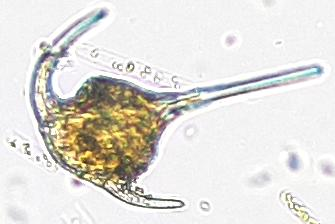
\includegraphics[width=\linewidth]{latex/figures/00_26_15_300342_10.jpg}
            \caption{\textit{Tripos} spp. (PlanktoScope)}
            \label{fig:tripos-ps}
        \end{subfigure} &
        \begin{subfigure}[b]{0.49\linewidth}
            \centering
            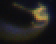
\includegraphics[width=\linewidth]{latex/figures/20231003_162111.225.0.png}
            \caption{\textit{Tripos} spp.\ \ \ \ \ \ \ \ \ \ \  (CPICS)}
            \label{fig:tripos-cpics}
        \end{subfigure} \\
        \begin{subfigure}[b]{0.49\linewidth}
            \centering
            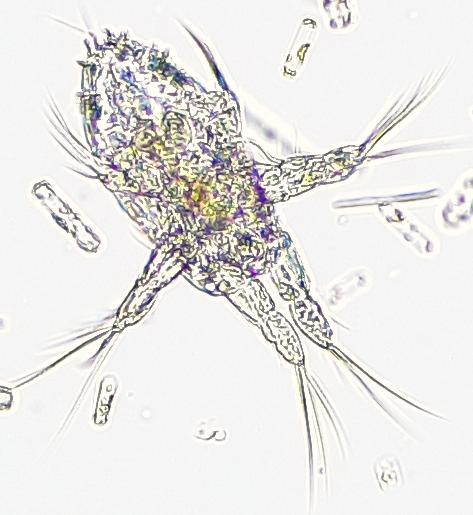
\includegraphics[width=\linewidth]{latex/figures/10_14_13_237354_14.jpg}
            \caption{Copepod naupli (PlanktoScope)}
            \label{fig:naupli-ps}
        \end{subfigure} &
        \begin{subfigure}[b]{0.49\linewidth}
            \centering
            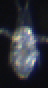
\includegraphics[height=\linewidth, angle=90,origin=c]{latex/figures/20230925_115158.468.0.png}
            \caption{Copepod naupli \ \ \ \ \ \ \ \ \ \ \  (CPICS)}
            \label{fig:naupli-cpics}
        \end{subfigure}
    \end{tabular}
    \caption{Examples and comparison of images from the PlanktoScope and CPICS. PlanktoScope images (a, c) have high resolution for small organisms and a light background. CPICS images (b, d) have lower resolution, but the throughput of the method is higher.}
    \label{fig:plankton-img}
\end{figure}

Samples for the PlanktoScope were taken with a plankton net from the shore in Drøbak, the Oslofjord, Norway (59.6635 N, 10.6256 E). The samples were pre-filtered through a 200 µm mesh sieve, and run through the PlanktoScope. The CPICS was deployed from a pier in Drøbak in October 2023. Both imagers have a built-in segmentation and feature extraction, which isolate regions of interest from the images and create metadata with, e.g., the size and shape of objects. The segmented images were manually classified in the Ecotaxa web portal (\hyperlink{https://ecotaxa.obs-vlfr.fr/}{https://ecotaxa.obs-vlfr.fr/}). For the PlanktoScope images, we used a small validated subset consisting of 2,061 images with 14 different categories. For the CPICS, we used all the validated data from the deployment, amounting to 222,000 images with 81 different categories.

\subsubsection{Image preprocessing}

The segmentation process in both imagers result in images of different dimensions, depending on the size and shape of the imaged object. However, most deep learning image classification methods require input images to be square with a specific resolution (REF). A common strategy is simply to reshape and resize the image to the right dimensions (REF), but this distorts the original shape of the object of interest, which could be important for correctly classifying plankton (REF?). Instead, we opted to resize only the largest dimension of the image to the correct resolution, and then pad the smallest dimension with the median edge color of the image. Since the images have an uniform light or dark background, the padding does not have a visible border, and should affect the classification minimally.


%
% =========================================================================

% =========================================================================
%
% Janita writes here
%
% =========================================================================

% =========================================================================
%
% Even writes here
%
% =========================================================================